\section{Results from Prior NSF Support}

PI Pollard brings decades of experience in grasping and manipulation analysis and experience working with various robotic hands and systems.   PI Coros brings experience in optimal design of creative, complex mechanisms to accomplish user specified tasks, as well as 10 years of experience in control algorithms for complex tasks.     This combination of skills is critical for designing and creating robot hands with the capability and skills to grasp and manipulate robustly in complex, real-world scenarios where humans and robots live and work together.

\begin{figure}
\begin{center}
{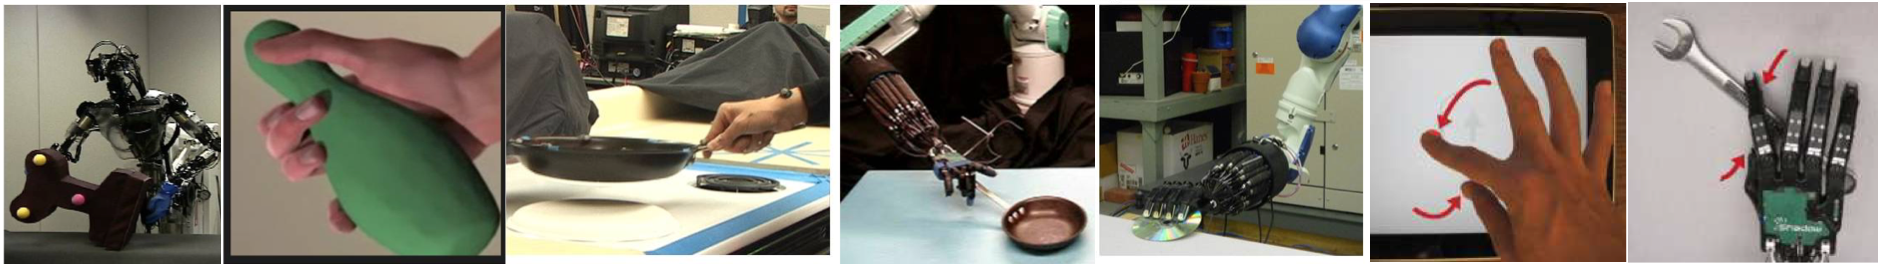
\includegraphics[width=\linewidth]{./figs/nspPrior}}
\end{center}
\vspace*{-0.2in}
\caption{Examples show prior research of PI Pollard in transfer of grasp and manipulation tasks, grasp planning with preparatory manipulation, and teleManipulation.}
\label{fig:nspPrior}
\end{figure}

\paragraph{Pollard's prior work on physics-based grasping and manipulation.} 
PI Pollard has extensive experience in grasp and manipulation planning, transfer, and optimization (Figure \ref{fig:nspPrior}).   She has developed algorithms for grasping and manipulation that allow fast transfer of examples from human to robot and generalization to varying object geometries in a manner that is both fast and provides bounds on performance \cite{pollard2004closure,Pollard:WAFR02,pollard2005physically,Li:graspDB07}.   She and her students have performed numerous human subjects studies to better understand the complex process of grasping in real-world situations \cite{Chang:2009,Chang:JMB10,illing2014changing,liu2016annotating} and followed up with more highly capable robot planning algorithms and quality metrics that function well for robot grasping in the presence of uncertainties \cite{Chang:ICRA10,Kappler:2012,kim2013physically}.   She has studied human-in-the-loop manipulation (teleManipulation) \cite{Toh:2012,chung2015quadratic,Kim:CGA11} and examined anatomical considerations of the human hand that may lead to better robot hand designs \cite{pollard2002tendon,fu2006importance,Chang:twoAxis08,Chang:CoR06,Chang:AoR06}.


\paragraph{Results from Prior NSF Support.}
Pollard has been funded by NSF awards \emph{CCF: Capturing and Animating the Human Hand: Robust Recovery of Hand-Object Interactions} NSF CCF0702443 (PI:  Pollard  6/07 - 5/11, \$325,000)  and \emph{CGV: Small: Simulation Motion Capture of Dexterous Manipulation} NSF IIS1218182 (PI:  Pollard  8/12 - 7/16, \$499,838).
{\bf Intellectual Merit:}  Results include taxonomies of everyday grasps, manipulations, and manipulation actions prior to grasping, findings on rotation prior to grasping, a novel algorithm for planning robotic tasks with preparatory manipulation, quality metrics for grasping that reflect real-world uncertainties and physics, robust
algorithms for capturing human hand skeletal structure, fast algorithms for simulation of deformable systems, a novel interactive system for guiding
simulations, a system for robot teleManipulation using multitouch, and an investigation of new
representations for motion that are meaningful across 
individuals and species (including robots).  This award resulted in the following
publications
\cite{liu2016annotating,chung2015quadratic,Liu2014,illing2014changing,kim2013physically,Toh:2012,Chang:2014,Gatesy:2011,Kappler:2012,Kim:ToG11,Kim:CGA11,Koonjul:ICRA11,Chang:JMB10,Chang:ICRA10,Kappler:Humanoids10,Chang:2009,Chang:twoAxis08,Chang:Humanoids08}.
{\bf Broader Impact:}  In addition to top venues in Robotics and Computer Graphics, results
have been published in the Journal of Motor Behavior, the Journal of
Biomechanics, the Journal of Theoretical Biology, and
in the book ``The Human Hand: A Source of Inspiration for
Robotic Hands.''  These grants supported two female PhD students, Lillian Chang and Yuzuko Nakamura,
whose dissertations contained many of the core research findings.  They also provided partial support for four masters students (two female), three undergraduates (two female),
and one postdoc.

\begin{figure}
\begin{center}
{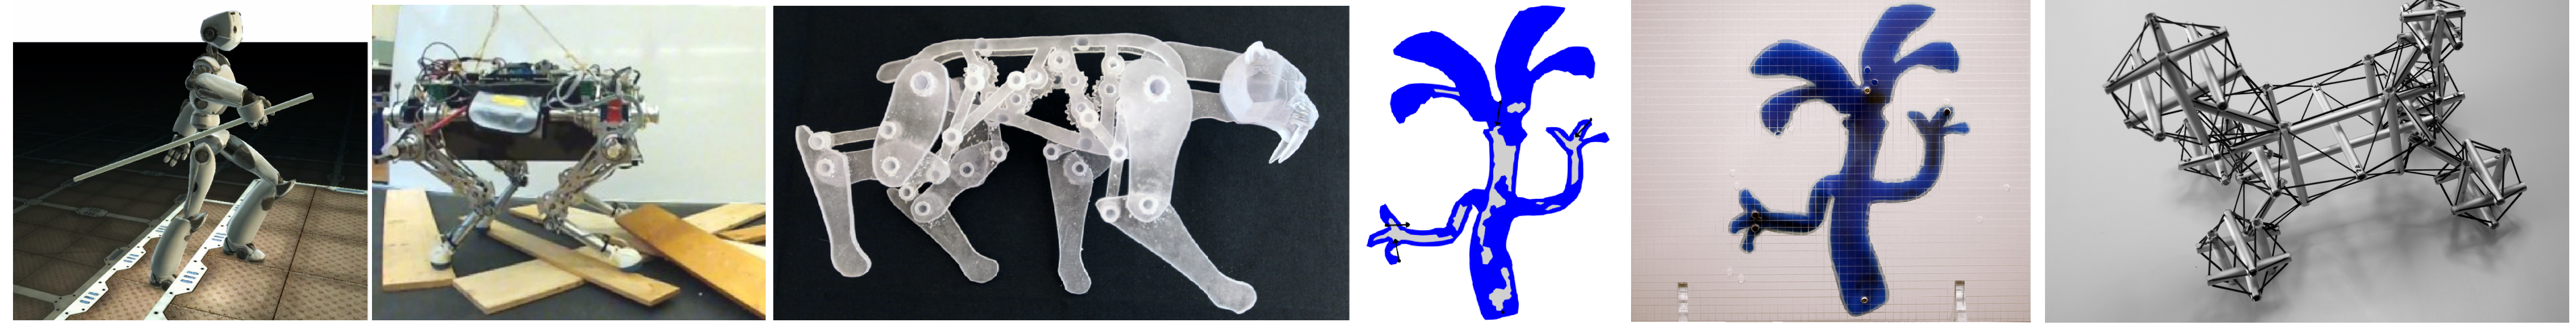
\includegraphics[width=\linewidth]{./figs/corosPrior}}
\end{center}
\vspace*{-0.2in}
\caption{Examples show prior research conducted by PI Coros in control methods for locomotion and manipulation, computational design of complex mechanical structures and digital fabrication.}
\label{fig:corosPrior}
\end{figure}

\paragraph{Coros's prior work on computational design and digital fabrication.} PI Coros has extensive experience in computer animation, robotics, computational design and digital fabrication, which are all areas of crucial importance for this proposal. Within the field of computer animation, the PI has developed physics-based methods that enable virtual actors to move autonomously using the same principles that underlie human and animal motions \cite{Yin08,Coros08,Coros09,Coros2010,Coros2011}. The PI extended these motor control models to apply them to \emph{StarlETH}, a dog-sized quadrupedal robot \cite{Gehring2015,Gehring2014,Gehring2013}. In addition to this line of work, the PI is investigating mathematical models and computational approaches to significantly simplify challenging design tasks that traditionally require a great deal of domain-specific knowledge. For example, he has developed several computational design systems that allow casual users to quickly design 3D printable mechanical automata \cite{Coros2013,Thomaszewski14CDL,Megaro14Chacra,Bacher2015}. Such complex mechanical assemblies combine geometric features, functionality and motion through a complex set of kinematic relationships and are notoriously difficult to design with traditional approaches. The PI's research has also ventured into the domain of multi-material 3D printing. For example, the goal of one of his recent projects was to automatically determine the distribution of rigid and soft materials within 3D printed objects such that the way in which they deform under the influence of external forces can be controlled \cite{Skouras2013}. This work complements other research efforts aimed at controlling the elastic properties of fabricated objects \cite{Gauge2014,Jesus2015} and builds on the soft body simulation models investigated by Coros and his colleagues \cite{Coros2012,Hahn2012,Schumacher2012}. Building on this body of work, this proposal will enable the design of a new class of robotic hands that are specifically designed for dexterous manipulation tasks.

\paragraph{Results from Prior NSF Support.} PI Coros is an NSF beginning investigator with no prior support.

